\section{Soorten netwerken}

\textit{In dit hoofdstuk wordt er onderzocht welke verschillende netwerken er gebruikt worden in bestaande implementaties. Hierbij wordt zowel de definitie van soorten en de selectie van implementaties gebruikt uit de resultaten van het vooronderzoek.}

"De distributie van informatie en het probleem van wederzijdse overeenstemming over een consistente staat van het netwerk vormt een uitdaging, zeker in de aanwezigheid van zelfzuchtige en/of kwaadwillende deelnemers" - \citet{7423672}. Het is een uitdaging die bekend staat als het Byzantine Generals' Problem, en is beschreven door \citet{lamport1982byzantine}. Het stelt dat het essentieel is voor een betrouwbaar computersysteem om te kunnen gaan met fouten die optreden in een of meer van de componenten, waardoor het kan voorkomen dat er conflicterende informatie verstuurd wordt naar de andere componenten van het systeem. In hoeverre een computersysteem hiermee om kan gaan wordt de \acrfull{BFT} genoemd en wordt aangeduid als: $ f = [\frac{N - 1}{t}] $ waarbij \(N\) componenten van een computersysteem zijn en \(t\) de foutieve componenten.

In blockchain implementaties zijn de componenten die onbetrouwbaar zijn de deelnemers van het peer-to-peer netwerk. Het soort netwerk is dan ook verbonden met de manier waarop consensus bereikt wordt tussen de deelnemers van het netwerk en is getypeerd als het consensus protocol dat geïmplementeerd is.

\newpage

\subsection{Proof of Work}
\label{chapter-proof-of-work}
De originele implementatie van Blockchain technologie is gepresenteerd door \citet{nakamoto2008bitcoin} in \textit{"Bitcoin: A peer-to-peer electronic cash system"}. Het maakt gebruik van een algoritme genaamd \acrfull{PoW} om consensus te bereiken. Hierbij gaat het om het oplossen van een wiskundig probleem $Y \in \mathbb{N} < f(X + n)$ waarbij $f$ een hash functie is, $n$ de \gls{nonce}, $X$ de data en $Y$ de \gls{difficulty}.

\begin{wrapfigure}{r}{0.5\textwidth}
  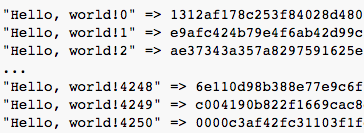
\includegraphics[width=0.5\textwidth, height=25mm]{proof-of-work}
  \caption{Werking Proof-of-Work, van \citet{ProofofWork}. Wanneer de eerste vier bits ($Y = 4$) van de hash 0 zijn is de proef opgelost. }
  \label{proof-of-work}    
\end{wrapfigure}
In het geval van Bitcoin is de $Y$ waarde een getal die aanduid wat de \gls{difficulty} is om de hash te berekenen en wordt de $X$ waarde incrementeel opgehoogd. Een voorbeeld is gegeven in fig. \ref{proof-of-work}. Dit proces zorgt ervoor dat de integriteit van de data in een block op de Blockchain bewaakt wordt. Wanneer een kwaadwillende deelnemer aan het netwerk de data van een block wilt aanpassen die reeds opgenomen is in de Blockchain, kan er via het \acrshort{PoW} makkelijk gevalideerd worden of het block invalide is.

Daarnaast beschrijft de bedenker van het protocol, Satoshi Nakamoto, het \acrshort{PoW} algoritme als 'one-CPU-one-vote'. Aangezien het gebruikte hashing algoritme geen limitaties stelt tot de zogeheten \gls{voting_power} van een deelnemer in het netwerk creëert het gunstige omstandigheden voor high-end GPU eigenaren tegenover high-end CPU eigenaren \citep[p.~2]{van2013cryptonote}.

\textbf{Monero} maakt gebruik van het CryptoNight algoritme \citep{noether2014monero}, een implementatie gebaseerd op CryptoNote, waarin gebruik gemaakt wordt van een egalitair Proof of Work \citep[p.~11]{van2013cryptonote}. In contrast met het Bitcoin protocol Proof of Work algoritme is het ontworpen om inefficiënt berekenbaar te zijn op een GPU, waardoor er gelijke kansen zijn voor de deelnemers van het netwerk die het mining proces uitvoeren.

\newpage
\subsection{Proof of Stake}

"Een eerste overweging met betrekking tot de werking van blockchain protocollen gebaseerd op Proof of Work -- zoals Bitcoin -- is de energie benodigd voor hun uitvoering." - \citet{kiayias2017ouroboros}.
In een onderzoek gedaan door \citeauthor{ODwyer:Bitcoin} in \citeyear{ODwyer:Bitcoin} naar het energieverbruik van het Bitcoin mining netwerk is geschat dat onder redelijke omstandigheden het netwerk gelijk stond met het energiegebruik van Ierland. Om deze reden zijn er onderzoeken en experimenten gedaan naar alternatieve consensus algoritmes. \acrfull{PoS} is een consensus algoritme waarbij, in plaats van het verspillen van elektriciteit om zware rekenkundige problemen op te lossen, een deelnemer geselecteerd wordt om het volgende blok te genereren (doorgaans \gls{minting} genoemd) op basis van willekeurige selectie en rijkdom of leeftijd (i.e., de stake).

\paragraph{Cardano} maakt gebruik van \acrshort{PoS} waarbij iedere deelnemer van het netwerk met een positief balans (e.g. stake) als stakeholders gezien worden. Om uitgekozen te worden om een nieuw block te genereren moet een stakeholder geselecteerd worden als \gls{slot_leader}. De implementatie verdeelt de fysieke tijd in tijdvakken en elke tijdvak is verdeeld in slots. Voor elke slot wordt een \gls{slot_leader} verkozen, die verantwoordelijk is voor het produceren van één blok. Niet alle deelnemers van het netwerk, bijvoorbeeld die minder dan 2\% van de totale circulatie van \glspl{token} hebben, worden geselecteerd om benoemd te worden tot \gls{slot_leader}. Deze groep van deelnemers maken deel uit van de \glspl{elector} groep. \Glspl{elector} verkiezen nieuwe \glspl{slot_leader} gedurende het huidige tijdsvak, waarna er een selectie gemaakt wordt en de nieuwe \glspl{slot_leader} vaststaan voor het volgende tijdsvak. Hoe meer \gls{stake} een deelnemer heeft, hoe groter de kans dat zij uitgekozen wordt om een \gls{slot_leader} te worden in het volgende tijdsvak. De \gls{slot_leader} luistert naar transacties die aangekondigd worden door andere nodes, bundelt ze in een nieuw block, signeert het met zijn private key en publiceert het block in het netwerk \citep{cardano_wiki:proof_of_stake}.

\paragraph{EOS} is een implementatie die gebruik maakt van \acrfull{DPoS} om consensus te bereiken. Het grote verschil tussen \acrshort{DPoS} en \acrshort{PoS}; in een \acrshort{PoS} systeem is elke deelnemer die \gls{stake} heeft maakt onderdeel uitmaken van het validatie- en consensusproces. Met \acrshort{DPoS} kan elke deelnemer die \gls{stake} heeft andere deelnemers verkiezen die onderdeel uitmaken van het validatie- en consensusproces \citep{steemit:eos_dpos}. In contrast met het \acrshort{PoW} algoritme is er geen competitie voor het produceren van een block, maar wordt er samengewerkt om een block te produceren.